\documentclass[tikz,border=2cm]{standalone}
\usetikzlibrary {arrows.meta}
\definecolor{pastelblue}{rgb}{0.68, 0.78, 0.81}
\definecolor{pastelyellow}{rgb}{0.99, 0.99, 0.59}
\definecolor{pastelpink}{rgb}{1.0, 0.82, 0.86}
\newif\ifimportant
\importanttrue
\begin{document}
    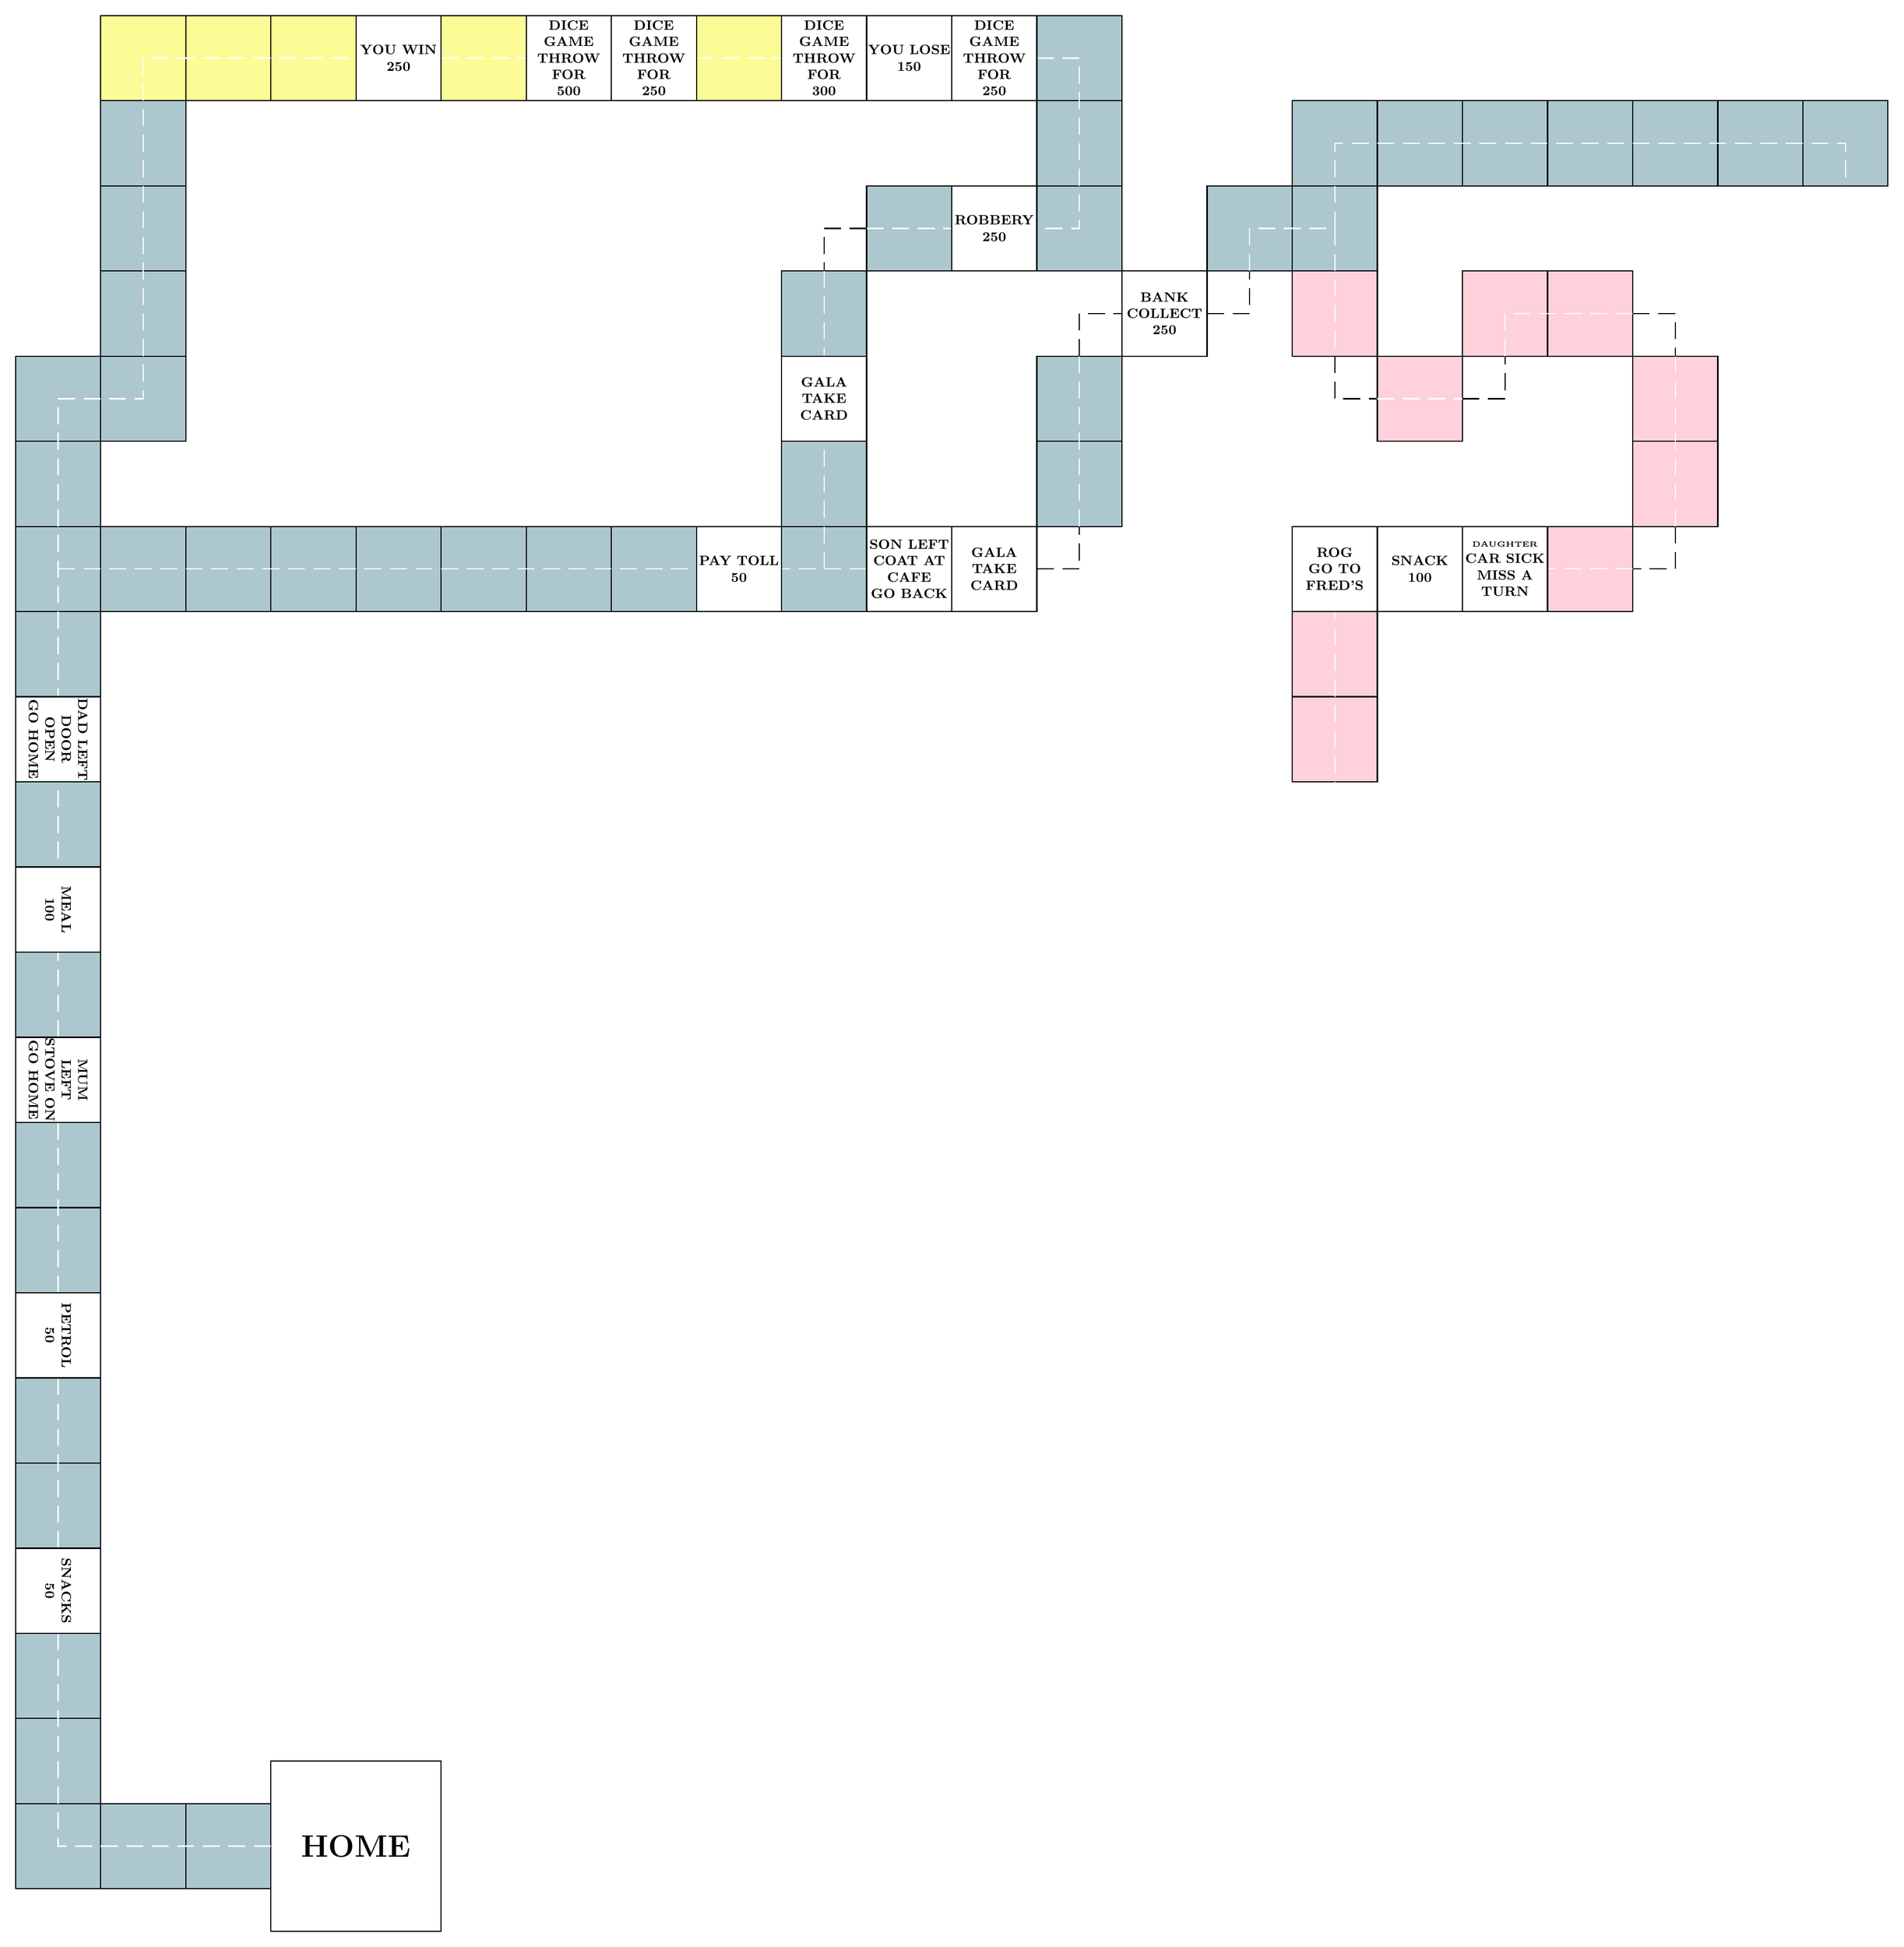
\begin{tikzpicture}
        [every node/.style={rectangle,draw=black,thick,inner sep=0pt,align=center},
        home-square/.style={minimum size=4cm,text width=4cm,font=\huge\bfseries},
        blue-square/.style={fill=pastelblue,minimum size=2cm,text width=2cm,font=\huge\bfseries,text=white},
        yellow-square/.style={fill=pastelyellow,minimum size=2cm,text width=2cm,font=\huge\bfseries,text=white},
        pink-square/.style={fill=pastelpink,minimum size=2cm,text width=2cm,font=\huge\bfseries,text=white},
        white-square/.style={minimum size=2cm,text width=2cm,font=\small\bfseries},
        whiteroad/.style={dash pattern=on 4mm off 2mm,thick,white},
        blackroad/.style={dash pattern=on 4mm off 2mm,thick}
        ]
        \node[home-square] (node-0) at (0, 0) {HOME};
        \node[blue-square] (node-1) at (-3, 0) {\ifimportant 1 \fi};
        \node[blue-square] (node-2) at (-5, 0) {\ifimportant 2 \fi};
        \node[blue-square] (node-3) at (-7, 0) {\ifimportant 3 \fi};
        \node[blue-square] (node-4) at (-7, 2) {\ifimportant 4 \fi};
        \node[blue-square] (node-5) at (-7, 4) {\ifimportant 5 \fi};
        \node[blue-square] (node-7) at (-7, 8) {\ifimportant 7 \fi};
        \node[blue-square] (node-8) at (-7, 10) {\ifimportant 8 \fi};
        \node[blue-square] (node-10) at (-7, 14) {\ifimportant 10 \fi};
        \node[blue-square] (node-11) at (-7, 16) {\ifimportant 11 \fi};
        \node[blue-square] (node-13) at (-7, 20) {\ifimportant 13 \fi};
        \node[blue-square] (node-15) at (-7, 24) {\ifimportant 15 \fi};
        \node[blue-square] (node-17) at (-7, 28) {\ifimportant 17 \fi};
        \node[blue-square] (node-18) at (-7, 30) {\ifimportant 18 \fi};
        \node[blue-square] (node-19) at (-7, 32) {\ifimportant 19 \fi};
        \node[blue-square] (node-20) at (-7, 34) {\ifimportant 20 \fi};
        \node[blue-square] (node-21) at (-5, 34) {\ifimportant 21 \fi};
        \node[blue-square] (node-22) at (-5, 36) {\ifimportant 22 \fi};
        \node[blue-square] (node-23) at (-5, 38) {\ifimportant 23 \fi};
        \node[blue-square] (node-24) at (-5, 40) {\ifimportant 24 \fi};
        \node[yellow-square] (node-25) at (-5, 42) {\ifimportant 25 \fi};
        \node[yellow-square] (node-26) at (-3, 42) {\ifimportant 26 \fi};
        \node[yellow-square] (node-27) at (-1, 42) {\ifimportant 27 \fi};
        \node[yellow-square] (node-29) at (3, 42) {\ifimportant 29 \fi};
        \node[yellow-square] (node-32) at (9, 42) {\ifimportant 32 \fi};
        \node[blue-square] (node-36) at (17, 42) {\ifimportant 36 \fi};
        \node[blue-square] (node-37) at (17, 40) {\ifimportant 37 \fi};
        \node[blue-square] (node-38) at (17, 38) {\ifimportant 38 \fi};
        \node[blue-square] (node-40) at (13, 38) {\ifimportant 40 \fi};
        \node[blue-square] (node-41) at (11, 36) {\ifimportant 41 \fi};
        \node[blue-square] (node-43) at (11, 32) {\ifimportant 43 \fi};
        \node[blue-square] (node-44) at (-5, 30) {\ifimportant 44 \fi};
        \node[blue-square] (node-45) at (-3, 30) {\ifimportant 45 \fi};
        \node[blue-square] (node-46) at (-1, 30) {\ifimportant 46 \fi};
        \node[blue-square] (node-47) at (1, 30) {\ifimportant 47 \fi};
        \node[blue-square] (node-48) at (3, 30) {\ifimportant 48 \fi};
        \node[blue-square] (node-49) at (5, 30) {\ifimportant 49 \fi};
        \node[blue-square] (node-50) at (7, 30) {\ifimportant 50 \fi};
        \node[blue-square] (node-52) at (11, 30) {\ifimportant 52 \fi};
        \node[blue-square] (node-55) at (17, 32) {\ifimportant 55 \fi};
        \node[blue-square] (node-56) at (17, 34) {\ifimportant 56 \fi};
        \node[blue-square] (node-58) at (21, 38) {\ifimportant 58 \fi};
        \node[blue-square] (node-59) at (23, 38) {\ifimportant 59 \fi};
        \node[pink-square] (node-60) at (23, 36) {\ifimportant 60 \fi};
        \node[pink-square] (node-61) at (25, 34) {\ifimportant 61 \fi};
        \node[pink-square] (node-62) at (27, 36) {\ifimportant 62 \fi};
        \node[pink-square] (node-63) at (29, 36) {\ifimportant 63 \fi};
        \node[pink-square] (node-64) at (31, 34) {\ifimportant 64 \fi};
        \node[pink-square] (node-65) at (31, 32) {\ifimportant 65 \fi};
        \node[pink-square] (node-66) at (29, 30) {\ifimportant 66 \fi};
        \node[pink-square] (node-70) at (23, 28) {\ifimportant 70 \fi};
        \node[pink-square] (node-71) at (23, 26) {\ifimportant 71 \fi};
        \node[blue-square] (node-72) at (23, 40) {\ifimportant 72 \fi};
        \node[blue-square] (node-73) at (25, 40) {\ifimportant 73 \fi};
        \node[blue-square] (node-74) at (27, 40) {\ifimportant 74 \fi};
        \node[blue-square] (node-75) at (29, 40) {\ifimportant 75 \fi};
        \node[blue-square] (node-76) at (31, 40) {\ifimportant 76 \fi};
        \node[blue-square] (node-77) at (33, 40) {\ifimportant 77 \fi};
        \node[blue-square] (node-78) at (35, 40) {\ifimportant 78 \fi};
        \draw[whiteroad] (-2, 0) -- (-7, 0) -- (-7, 34) -- (-5, 34) -- (-5, 41);
        \draw[whiteroad] (-5, 41) -- (-5, 42) -- (0, 42);
        \draw[whiteroad] (2, 42) -- (4, 42);
        \draw[whiteroad] (8, 42) -- (10, 42);
        \draw[whiteroad] (16, 42) -- (17, 42) -- (17, 38) -- (12, 38);
        \draw[blackroad] (12, 38) -- (11, 38) -- (11, 37);
        \draw[whiteroad] (11, 37) -- (11, 30);
        \draw[whiteroad] (-7, 30) -- (16, 30);
        \draw[blackroad] (16, 30) -- (17, 30) -- (17, 31);
        \draw[whiteroad] (17, 31) -- (17, 35);
        \draw[blackroad] (17, 35) -- (17, 36) -- (18, 36);
        \draw[blackroad] (20, 36) -- (21, 36) -- (21, 37);
        \draw[whiteroad] (21, 37) -- (21, 38) -- (23, 38) -- (23, 35);
        \draw[blackroad] (23, 35) -- (23, 34) -- (24, 34);
        \draw[whiteroad] (24, 34) -- (26, 34);
        \draw[blackroad] (26, 34) -- (27, 34) -- (27, 35);
        \draw[whiteroad] (27, 35) -- (27, 36) -- (30, 36);
        \draw[blackroad] (30, 36) -- (31, 36) -- (31, 35);
        \draw[whiteroad] (31, 35) -- (31, 31);
        \draw[blackroad] (31, 31) -- (31, 30) -- (30, 30);
        \draw[whiteroad] (30, 30) -- (23, 30) -- (23, 24);
        \draw[whiteroad] (23, 38) -- (23, 40) -- (35, 40) -- (35, 39);
        \node[white-square,rotate=270] (node-6) at (-7, 6) {SNACKS\\50};
        \node[white-square,rotate=270] (node-9) at (-7, 12) {PETROL\\50};
        \node[white-square,rotate=270] (node-12) at (-7, 18) {MUM LEFT\\STOVE ON\\GO HOME};
        \node[white-square,rotate=270] (node-14) at (-7, 22) {MEAL\\100};
        \node[white-square,rotate=270] (node-16) at (-7, 26) {DAD LEFT\\DOOR OPEN\\GO HOME};
        \node[white-square] (node-28) at (1, 42) {YOU WIN\\250};
        \node[white-square] (node-30) at (5, 42) {DICE GAME\\THROW FOR\\500};
        \node[white-square] (node-31) at (7, 42) {DICE GAME\\THROW FOR\\250};
        \node[white-square] (node-33) at (11, 42) {DICE GAME\\THROW FOR\\300};
        \node[white-square] (node-34) at (13, 42) {YOU LOSE\\150};
        \node[white-square] (node-35) at (15, 42) {DICE GAME\\THROW FOR\\250};
        \node[white-square] (node-39) at (15, 38) {ROBBERY\\250};
        \node[white-square] (node-42) at (11, 34) {GALA\\TAKE\\CARD};
        \node[white-square] (node-51) at (9, 30) {PAY TOLL\\50};
        \node[white-square] (node-53) at (13, 30) {SON LEFT\\COAT AT\\CAFE\\GO BACK};
        \node[white-square] (node-54) at (15, 30) {GALA\\TAKE\\CARD};
        \node[white-square] (node-57) at (19, 36) {BANK\\COLLECT\\250};
        \node[white-square] (node-67) at (27, 30) {{\tiny DAUGHTER}\\CAR SICK\\MISS A\\TURN};
        \node[white-square] (node-68) at (25, 30) {SNACK\\100};
        \node[white-square] (node-69) at (23, 30) {ROG\\GO TO\\FRED'S};
    \end{tikzpicture}
\end{document}